\documentclass[a4paper]{article}
\usepackage{graphicx}
\title{Deletion Logic - SIPSL}
\author{guic}
\date{October 2010}
\begin{document}
	\small
	\maketitle
\section{Message Lifecycle}

\subsection{Creation}

The creation is done in different ways:

\begin{itemize}
   \item Incoming from network
   \item Create internally a request, reply or operation
\end{itemize}

\subsection{Incoming from network}

The buffer is used to create message. The message is inserted into the global message table. 
The key for the message table is the address of the message.

\begin{verbatim}
MESSAGE* newmessage=0x0;
CREATENEWMESSAGE_EXT(newmessage, incomingbuffer, socket,
    echoclientaddress, networksourcepoint)
\end{verbatim}

Message key is made by the following information:
\begin{verbatim}

  key = <address of message integer><creation timestamp>
  example:
    85b4d501286797872880071

\end{verbatim}
	
\subsection{Create internally a request, reply or operation}
	
The message is copied from another exiting message. Only the buffer and other info is copied, the headers are left empty; this means that there are no copy constructors.	
	
\begin{verbatim}
CREATEMESSAGE(newmessage, sourcemessage, generatingpoint)
\end{verbatim}

The source message can be a request or reply and the new message also (there is not constraint).

\section{Deletion control}

\subsection{Message lock and lock table}

The purpose of the lock and the lock table is because some messages may require to remain allocated during the entire lifecycle of the call,
other messages can be deleted immediately after being sent.

The transmission layer will check the lock, if the message is locked it will not be deleted. 
All the message in the lock table will be deleted once the deletion of the call object has been requested, so it is not mandatory to unlock messages an delete once they are not useful
(but it is recommended though).

The lock must be checked before deleting the message. The deletion is done by PURGEMESSAGE which will also remove it from the global message table:
\begin{verbatim}
PURGEMESSAGE(message)
\end{verbatim}

When the lock is set, the message must also be stored in the locked message table:
\begin{verbatim}
message->setLock();
call_oset->insertLockedMessage(message);
\end{verbatim}
The table is local to the call. If the message is unlocked it must also be removed from the table.

\section{Messages lifecycle cases}

\subsection{INVITE A - incoming invite}

\begin {itemize}
\item invite arrives in SUDP, message is created
\item message traverses the SIPENGINE
\item message traverses the SL\_CC
\begin {itemize}
\item CALL\_OSET is created
\item message is sent to COMAP which will find the correct SL\_CO
\item COMAP will execute the SL\_CO::call
\begin {itemize}
\item SL\_CO::call will create the Invite Server Transaction State Machine TRNSCT\_SM\_INVITE\_SV
\item the message is stored into the Matrix and locked.
\end{itemize}
\end{itemize}
\end{itemize}

INVITE A is also stored locally in VALO.

The INVITE A is delete at the end of the call when the TRNSCT\_SM\_INVITE\_SV is deleted.

\subsection{100 TRY A - immediate reply by SIPSL to A}

The 100 TRY A is generated using INVITE A and deleted after transmission.

\subsection{INVITE B - outgoing invite}

\begin {itemize}
\item INVITE B is created in VALO (pointer is stored locally)
\item message traverses the SL\_CC
\begin {itemize}
\item CALL\_OSET is found
\item message is sent to COMAP which will find the correct SL\_CO
\item COMAP will execute the SL\_CO::call
\begin {itemize}
\item SL\_CO::call will create the Invite Client Transaction State Machine TRNSCT\_SM\_INVITE\_CL
\item the message is stored into the Matrix and locked.
\item the invite is duplicated and a copy is sent to ALARM (locked and stored in locked messages)
\end{itemize}
\end{itemize}
\end{itemize}

\subsection{INVITE B ALARM for retransmission}

\begin {itemize}
\item INVITE B ALARM arrives at the client state machine it is duplicated and set as operation "timer on"
\item The new INVITE B timer is locked and stored into the locked messages table
\item The incoming message is unlocked and sent to SUDP
\item SUDP will delete the message
\end{itemize}

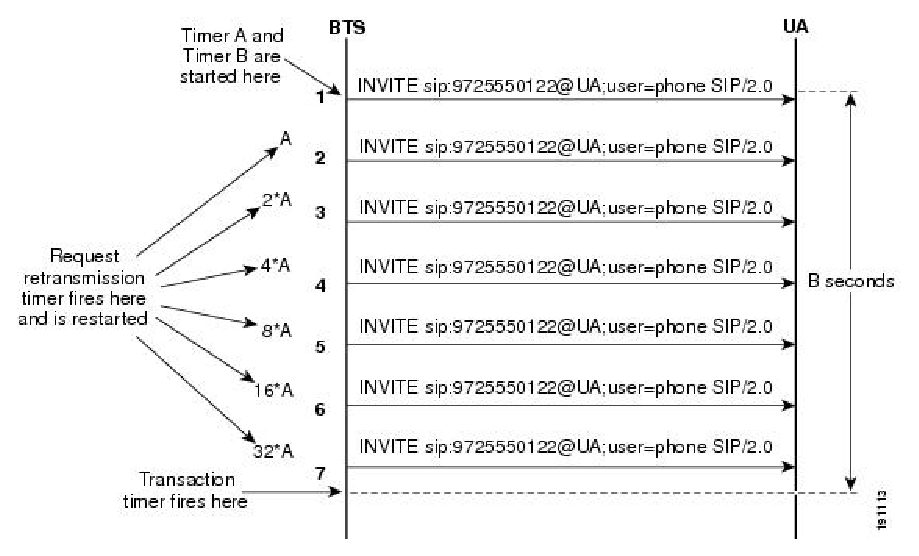
\includegraphics[width=90mm]{timerAlogic.eps}

\subsection{100 Try B}
\begin {itemize}
\item Message is modified to cancel the alarm
\item Message is sent to alarm
\item Message is deleted
\end{itemize}

\subsection{101 DIALOG ESTABLISHED B or 180 RINGING B}
\begin {itemize}
\item Message is duplicated into and changed into A side reply
\item Message is modified to cancel the alarm
\item Message is sent to alarm
\item Message is deleted
\end{itemize}

\subsection{101 DIALOG ESTABLISHED A or 180 RINGING A}
TO BE IMPLEMENTED
\begin {itemize}
\item Message is locked stored into the state machine as STOREMESS\_1\_2 for retransmission 
\item Message is sent
\end{itemize}

\subsection{200 OK B}
\begin {itemize}
\item Message is sent to ALO
\item Message is duplicated modified to cancel the alarm
\item Message is sent to alarm
\item Message is deleted
\item The copy is sent to ALO
\item ALO accesses the A\_Matrix of client state machine (INVITE A)
\item Message is duplicated
\item Message is modified to be a 200OK A with the 200OKB sdp part
\item Message is sent to sv
\item 200 OK B is deleted
\end{itemize}

IMPLEMENT THE resend to 200ok if ACK missing

\subsection{200 OK A}
\begin {itemize}
\item Message is stored into STOREMESS\_1\_3 for retranmission in case the INVITE A arrives again
\item Message is duplicated and sent to alarm in case the ACK A does not arrives
\item Massage is sent to A
\end{itemize}

\subsection{ACK A}
Ack comes to SL\_CC and a new state machine is created.
\begin {itemize}
\item Message is stored in the Matrix 
\item Message is sent to ALO
\item ALO creates the Ack B
\item Ack B arrives at client sm
\end{itemize}

\subsection{ACK B}
Ack comes to SL\_CC and a new state machine is created.
\begin {itemize}
\item Message is stored in the Matrix 
\item Message is sent to network
\end{itemize}

\subsection{200 OK B resend by B}
The 200 OK is repeated by B, the ACK b must be resent
\begin{itemize}
\item 200 OK arrives to INVITE client SM
\item the sm changes the CSEQ to ACK
\item the 200 ok is resent to client
\item ack client SM receives the 200 OK
\item the sm ack client resend the ack
\end{itemize}

\subsection{Timers table}

\begin{verbatim}

A Table of Timer Values

   Table 4 summarizes the meaning and defaults of the various timers
   used by this specification.

Timer    Value            Section               Meaning
----------------------------------------------------------------------
T1       500ms default    Section 17.1.1.1     RTT Estimate
T2       4s               Section 17.1.2.2     The maximum retransmit
                                               interval for non-INVITE
                                               requests and INVITE
                                               responses
T4       5s               Section 17.1.2.2     Maximum duration a
                                               message will
                                               remain in the network
Timer A  initially T1     Section 17.1.1.2     INVITE request retransmit
                                               interval, for UDP only
Timer B  64*T1            Section 17.1.1.2     INVITE transaction
                                               timeout timer
Timer C  > 3min           Section 16.6         proxy INVITE transaction
                           bullet 11            timeout
Timer D  > 32s for UDP    Section 17.1.1.2     Wait time for response
         0s for TCP/SCTP                       retransmits
Timer E  initially T1     Section 17.1.2.2     non-INVITE request
                                               retransmit interval,
                                               UDP only
Timer F  64*T1            Section 17.1.2.2     non-INVITE transaction
                                               timeout timer
Timer G  initially T1     Section 17.2.1       INVITE response
                                               retransmit interval
Timer H  64*T1            Section 17.2.1       Wait time for
                                               ACK receipt
Timer I  T4 for UDP       Section 17.2.1       Wait time for
         0s for TCP/SCTP                       ACK retransmits
Timer J  64*T1 for UDP    Section 17.2.2       Wait time for
         0s for TCP/SCTP                       non-INVITE request
                                               retransmits
Timer K  T4 for UDP       Section 17.1.2.2     Wait time for
         0s for TCP/SCTP                       response retransmits

                   Table 4: Summary of timers

\end{verbatim}

\pagebreak
\section{Call States}

\begin{verbatim}

                               |INVITE
                               |pass INV to TU
            INVITE             V send 100 if TU won't in 200ms
            send response+-----------+
                +--------|           |--------+101-199 from TU
                |        | Proceeding|        |send response
                +------->|           |<-------+
                         |           |          Transport Err.
                         |           |          Inform TU
                         |           |--------------->+
                         +-----------+                |
            300-699 from TU |     |2xx from TU        |
            send response   |     |send response      |
                            |     +------------------>+
                            |                         |
            INVITE          V          Timer G fires  |
            send response+-----------+ send response  |
                +--------|           |--------+       |
                |        | Completed |        |       |
                +------->|           |<-------+       |
                         +-----------+                |
                            |     |                   |
                        ACK |     |                   |
                        -   |     +------------------>+
                            |        Timer H fires    |
                            V        or Transport Err.|
                         +-----------+  Inform TU     |
                         |           |                |
                         | Confirmed |                |
                         |           |                |
                         +-----------+                |
                               |                      |
                               |Timer I fires         |
                               |-                     |
                               |                      |
                               V                      |
                         +-----------+                |
                         |           |                |
                         | Terminated|<---------------+
                         |           |
                         +-----------+

                     INVITE server transaction
                     
\end{verbatim}
\pagebreak
\begin{verbatim}

                               |INVITE from TU
             Timer A fires     |INVITE sent
             Reset A,          V                      Timer B fires
             INVITE sent +-----------+                or Transport Err.
               +---------|           |---------------+inform TU
               |         |  Calling  |               |
               +-------->|           |-------------->|
                         +-----------+ 2xx           |
                            |  |       2xx to TU     |
                            |  |1xx                  |
    300-699 +---------------+  |1xx to TU            |
   ACK sent |                  |                     |
resp. to TU |  1xx             V                     |
            |  1xx to TU  -----------+               |
            |  +---------|           |               |
            |  |         |Proceeding |-------------->|
            |  +-------->|           | 2xx           |
            |            +-----------+ 2xx to TU     |
            |       300-699    |                     |
            |       ACK sent,  |                     |
            |       resp. to TU|                     |
            |                  |                     |      NOTE:
            |  300-699         V                     |
            |  ACK sent  +-----------+Transport Err. |  transitions
            |  +---------|           |Inform TU      |  labeled with
            |  |         | Completed |-------------->|  the event
            |  +-------->|           |               |  over the action
            |            +-----------+               |  to take
            |              ^   |                     |
            |              |   | Timer D fires       |
            +--------------+   | -                   |
                               |                     |
                               V                     |
                         +-----------+               |
                         |           |               |
                         | Terminated|<--------------+
                         |           |
                         +-----------+

                     INVITE client transaction

end{verbatim}


\section{Call\_OSet lifecyle}

The deletion of the call\_oset is triggered using:
\begin{verbatim}
	COMAP::setDoaRequested(call_oset, message->getModulus());
\end{verbatim} 

\end{document}
